
%(BEGIN_QUESTION)
% Copyright 2011, Tony R. Kuphaldt, released under the Creative Commons Attribution License (v 1.0)
% This means you may do almost anything with this work of mine, so long as you give me proper credit

The purpose of this circuit is to maintain a constant current through the thermistor, so that $V_{out}$ will be an accurate representation of the thermistor's resistance (and therefore its temperature):

$$\includegraphics[width=15.5cm]{i01698x01.eps}$$

First, identify the necessary value for $R_{prg}$ in order to establish the thermistor's current at 145 microamps.

\vskip 10pt

Next, suppose we find one day that $V_{out}$ is 0 volts, even though the power supply to this circuit has been verified to be 24 VDC just as it should.  Identify the likelihood of each specified fault for this circuit.  Consider each fault one at a time (i.e. no coincidental faults), determining whether or not each fault could independently account for {\it all} measurements and symptoms in this circuit.

% No blank lines allowed between lines of an \halign structure!
% I use comments (%) instead, so that TeX doesn't choke.

$$\vbox{\offinterlineskip
\halign{\strut
\vrule \quad\hfil # \ \hfil & 
\vrule \quad\hfil # \ \hfil & 
\vrule \quad\hfil # \ \hfil \vrule \cr
\noalign{\hrule}
%
% First row
{\bf Fault} & {\bf Possible} & {\bf Impossible} \cr
%
\noalign{\hrule}
%
% Another row
$R_1$ failed open &  &  \cr
%
\noalign{\hrule}
%
% Another row
$R_2$ failed open &  &  \cr
%
\noalign{\hrule}
%
% Another row
$R_{prg}$ failed open &  &  \cr
%
\noalign{\hrule}
%
% Another row
Thermistor failed open &  &  \cr
%
\noalign{\hrule}
%
% Another row
Transistor failed open C-E &  &  \cr
%
\noalign{\hrule}
%
% Another row
$R_1$ failed shorted &  &  \cr
%
\noalign{\hrule}
%
% Another row
$R_2$ failed shorted &  &  \cr
%
\noalign{\hrule}
%
% Another row
$R_{prg}$ failed shorted &  &  \cr
%
\noalign{\hrule}
%
% Another row
Thermistor failed shorted &  &  \cr
%
\noalign{\hrule}
} % End of \halign 
}$$ % End of \vbox

Finally, identify the {\it next} diagnostic test or measurement you would make on this system.  Explain how the result(s) of this next test or measurement help further identify the location and/or nature of the fault.

\vskip 20pt \vbox{\hrule \hbox{\strut \vrule{} {\bf Suggestions for Socratic discussion} \vrule} \hrule}

\begin{itemize}
\item{} Explain how the opamp's connection to the two 2.2 k$\Omega$ resistors and to the NPN transistor forms a {\it negative feedback} system, although it appears to be positive feedback at first glance due to which side of the circuit the transistor is on.
\end{itemize}

\underbar{file i01698}
%(END_QUESTION)





%(BEGIN_ANSWER)

A current of 145 microamps through the thermistor will be 145 microamps through $R_2$ (assuming the opamp inputs draw negligible current).  Therefore, we need a voltage of 0.319 volts across $R_2$ (and by extension, across $R_1$ as well).

\vskip 10pt

In order to get the same current through $R_1$, we need $R_{prg}$ to be large enough that the whole supply voltage of 24 VDC is just enough to get 145 microamps through the series combination of $R_1$ and $R_{prg}$.  Thus, $R_1 + R_{prg}$ = 24 V / 145 $\mu$A = 165.52 k$\Omega$.  Subtracting $R_2$'s value of 2.2 kilo-ohms yields this result for the programming resistor:

\vskip 10pt

$R_{prg}$ = 163.32 k$\Omega$

\vskip 10pt

\noindent
{\bf Partial answer:}

% No blank lines allowed between lines of an \halign structure!
% I use comments (%) instead, so that TeX doesn't choke.

$$\vbox{\offinterlineskip
\halign{\strut
\vrule \quad\hfil # \ \hfil & 
\vrule \quad\hfil # \ \hfil & 
\vrule \quad\hfil # \ \hfil \vrule \cr
\noalign{\hrule}
%
% First row
{\bf Fault} & {\bf Possible} & {\bf Impossible} \cr
%
\noalign{\hrule}
%
% Another row
$R_1$ failed open &  & $\surd$ \cr
%
\noalign{\hrule}
%
% Another row
$R_2$ failed open &  &  \cr
%
\noalign{\hrule}
%
% Another row
$R_{prg}$ failed open &  &  \cr
%
\noalign{\hrule}
%
% Another row
Thermistor failed open &  &  \cr
%
\noalign{\hrule}
%
% Another row
Transistor failed open C-E & $\surd$ &  \cr
%
\noalign{\hrule}
%
% Another row
$R_1$ failed shorted &  &  \cr
%
\noalign{\hrule}
%
% Another row
$R_2$ failed shorted &  &  \cr
%
\noalign{\hrule}
%
% Another row
$R_{prg}$ failed shorted &  &  \cr
%
\noalign{\hrule}
%
% Another row
Thermistor failed shorted & $\surd$ &  \cr
%
\noalign{\hrule}
} % End of \halign 
}$$ % End of \vbox


%(END_ANSWER)





%(BEGIN_NOTES)

A $V_{out}$ of 0 volts means either the thermistor has shorted, or there is no current going through it.

% No blank lines allowed between lines of an \halign structure!
% I use comments (%) instead, so that TeX doesn't choke.

$$\vbox{\offinterlineskip
\halign{\strut
\vrule \quad\hfil # \ \hfil & 
\vrule \quad\hfil # \ \hfil & 
\vrule \quad\hfil # \ \hfil \vrule \cr
\noalign{\hrule}
%
% First row
{\bf Fault} & {\bf Possible} & {\bf Impossible} \cr
%
\noalign{\hrule}
%
% Another row
$R_1$ failed open &  & $\surd$ \cr
%
\noalign{\hrule}
%
% Another row
$R_2$ failed open & $\surd$ &  \cr
%
\noalign{\hrule}
%
% Another row
$R_{prg}$ failed open & $\surd$ &  \cr
%
\noalign{\hrule}
%
% Another row
Thermistor failed open &  & $\surd$ \cr
%
\noalign{\hrule}
%
% Another row
Transistor failed open C-E & $\surd$ &  \cr
%
\noalign{\hrule}
%
% Another row
$R_1$ failed shorted & $\surd$ &  \cr
%
\noalign{\hrule}
%
% Another row
$R_2$ failed shorted &  & $\surd$ \cr
%
\noalign{\hrule}
%
% Another row
$R_{prg}$ failed shorted &  & $\surd$ \cr
%
\noalign{\hrule}
%
% Another row
Thermistor failed shorted & $\surd$ &  \cr
%
\noalign{\hrule}
} % End of \halign 
}$$ % End of \vbox


%INDEX% Measurement, temperature: current mirror circuit for RTDs and thermistors
%INDEX% Troubleshooting review: electric circuits

%(END_NOTES)


